% Options for packages loaded elsewhere
\PassOptionsToPackage{unicode}{hyperref}
\PassOptionsToPackage{hyphens}{url}
%
\documentclass[
  letterpaper,
  ignorenonframetext,
  aspectratio=43,
  handout,
  12pt]{beamer}
\usepackage{pgfpages}
\setbeamertemplate{caption}[numbered]
\setbeamertemplate{caption label separator}{: }
\setbeamercolor{caption name}{fg=normal text.fg}
\beamertemplatenavigationsymbolsempty
% Prevent slide breaks in the middle of a paragraph
\widowpenalties 1 10000
\raggedbottom
\setbeamertemplate{part page}{
  \centering
  \begin{beamercolorbox}[sep=16pt,center]{part title}
    \usebeamerfont{part title}\insertpart\par
  \end{beamercolorbox}
}
\setbeamertemplate{section page}{
  \centering
  \begin{beamercolorbox}[sep=12pt,center]{part title}
    \usebeamerfont{section title}\insertsection\par
  \end{beamercolorbox}
}
\setbeamertemplate{subsection page}{
  \centering
  \begin{beamercolorbox}[sep=8pt,center]{part title}
    \usebeamerfont{subsection title}\insertsubsection\par
  \end{beamercolorbox}
}
\AtBeginPart{
  \frame{\partpage}
}
\AtBeginSection{
  \ifbibliography
  \else
    \frame{\sectionpage}
  \fi
}
\AtBeginSubsection{
  \frame{\subsectionpage}
}
\usepackage{lmodern}
\usepackage{amssymb,amsmath}
\usepackage{ifxetex,ifluatex}
\ifnum 0\ifxetex 1\fi\ifluatex 1\fi=0 % if pdftex
  \usepackage[T1]{fontenc}
  \usepackage[utf8]{inputenc}
  \usepackage{textcomp} % provide euro and other symbols
\else % if luatex or xetex
  \usepackage{unicode-math}
  \defaultfontfeatures{Scale=MatchLowercase}
  \defaultfontfeatures[\rmfamily]{Ligatures=TeX,Scale=1}
\fi
\usetheme[]{metropolis}
% Use upquote if available, for straight quotes in verbatim environments
\IfFileExists{upquote.sty}{\usepackage{upquote}}{}
\IfFileExists{microtype.sty}{% use microtype if available
  \usepackage[]{microtype}
  \UseMicrotypeSet[protrusion]{basicmath} % disable protrusion for tt fonts
}{}
\makeatletter
\@ifundefined{KOMAClassName}{% if non-KOMA class
  \IfFileExists{parskip.sty}{%
    \usepackage{parskip}
  }{% else
    \setlength{\parindent}{0pt}
    \setlength{\parskip}{6pt plus 2pt minus 1pt}}
}{% if KOMA class
  \KOMAoptions{parskip=half}}
\makeatother
\usepackage{xcolor}
\IfFileExists{xurl.sty}{\usepackage{xurl}}{} % add URL line breaks if available
\IfFileExists{bookmark.sty}{\usepackage{bookmark}}{\usepackage{hyperref}}
\hypersetup{
  hidelinks,
  pdfcreator={LaTeX via pandoc}}
\urlstyle{same} % disable monospaced font for URLs
\newif\ifbibliography
\usepackage{graphicx}
\makeatletter
\def\maxwidth{\ifdim\Gin@nat@width>\linewidth\linewidth\else\Gin@nat@width\fi}
\def\maxheight{\ifdim\Gin@nat@height>\textheight\textheight\else\Gin@nat@height\fi}
\makeatother
% Scale images if necessary, so that they will not overflow the page
% margins by default, and it is still possible to overwrite the defaults
% using explicit options in \includegraphics[width, height, ...]{}
\setkeys{Gin}{width=\maxwidth,height=\maxheight,keepaspectratio}
% Set default figure placement to htbp
\makeatletter
\def\fps@figure{htbp}
\makeatother
\setlength{\emergencystretch}{3em} % prevent overfull lines
\providecommand{\tightlist}{%
  \setlength{\itemsep}{0pt}\setlength{\parskip}{0pt}}
\setcounter{secnumdepth}{-\maxdimen} % remove section numbering
\usepackage{pgfpages}
\pgfpagesuselayout{2 on 1}
\providecommand{\tightlist}{%
\setlength{\itemsep}{0pt}\setlength{\parskip}{0pt}}
\makeatletter
\makeatother
\let\Oldincludegraphics\includegraphics
\renewcommand{\includegraphics}[2][]{\Oldincludegraphics[width=\textwidth,height=0.7\textheight,keepaspectratio]{#2}}
\newcommand{\highlight}[1]{%
  \colorbox{red!50}{$\displaystyle#1$}}
\ifluatex
  \usepackage{selnolig}  % disable illegal ligatures
\fi

\author{}
\date{}

\begin{document}

\begin{frame}{Continuum Mechanics}
\protect\hypertarget{continuum-mechanics}{}
Lecture 11 - Anisotropy

Dr.~Nicholas Smith

Wichita State University, Department of Aerospace Engineering

6 October, 2020
\end{frame}

\begin{frame}{schedule}
\protect\hypertarget{schedule}{}
\begin{itemize}
\tightlist
\item
  6 Oct - Anisotropy
\item
  8 Oct - Large Deformation
\item
  13 Oct - Anisotropy and Large Deformation
\item
  15 Oct - Exam Review
\item
  20 Oct - Exam 2
\end{itemize}
\end{frame}

\begin{frame}{outline}
\protect\hypertarget{outline}{}
\begin{itemize}
\tightlist
\item
  anisotropic materials
\item
  physical interpretation
\item
  material symmetries
\item
  experimental considerations
\end{itemize}
\end{frame}

\begin{frame}{anisotropic materials}
\protect\hypertarget{anisotropic-materials}{}
\begin{itemize}
\tightlist
\item
  Many materials exhibit different properties in different directions
\item
  Composites are one example, but many polymers have anisotropy due to
  crystallinity
\item
  Even some metals exhibit minor amounts of anisotropy due to grain
  boundaries and rolling
\item
  Wood is a common anisotropic material
\end{itemize}
\end{frame}

\begin{frame}{anisotropic materials}
\protect\hypertarget{anisotropic-materials-1}{}
\begin{figure}
\centering
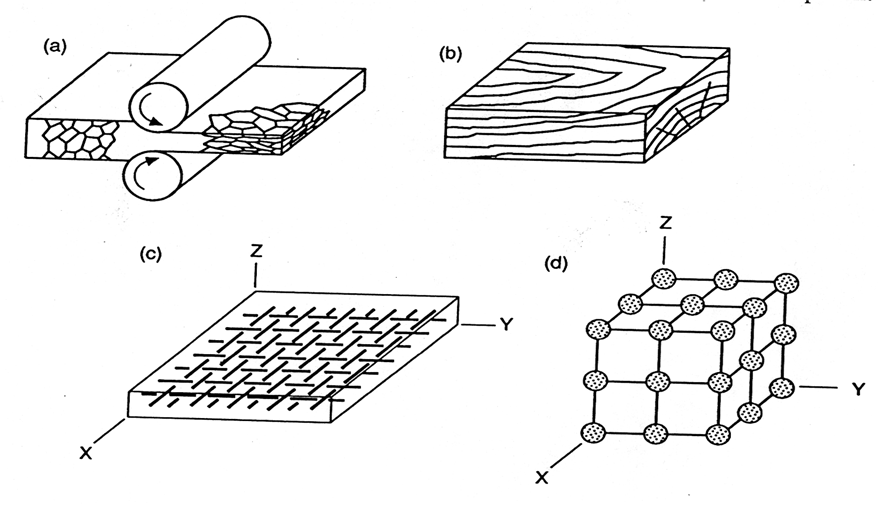
\includegraphics{../images/anisotropy.png}
\caption{image}
\end{figure}
\end{frame}

\begin{frame}{hooke's law}
\protect\hypertarget{hookes-law}{}
\begin{itemize}
\tightlist
\item
  Although it cannot be simplified as much as for isotropic materials,
  Hooke's Law still applies to linear anisotropic materials
  \[T_{ij} = C_{ijkl}E_{kl}\]
\end{itemize}
\end{frame}

\begin{frame}{hooke's law}
\protect\hypertarget{hookes-law-1}{}
\begin{itemize}
\tightlist
\item
  Or, written in ``engineering'' form \[\begin{bmatrix}
    T_{11}\\ T_{22} \\ T_{33} \\ T_{23} \\ T_{13} \\ T_{12}
    \end{bmatrix}
    = \begin{bmatrix}
    C_{1111} & C_{1122} & C_{1133} & C_{1123} & C_{1113} & C_{1112} \\
    C_{1122} & C_{2222} & C_{2233} & C_{2223} & C_{1322} & C_{1222} \\
    C_{1133} & C_{2233} & C_{3333} & C_{2333} & C_{1333} & C_{1233} \\
    C_{1123} & C_{2223} & C_{2333} & C_{2323} & C_{1323} & C_{1223} \\
    C_{1113} & C_{1322} & C_{1333} & C_{1323} & C_{1313} & C_{1213} \\
    C_{1112} & C_{1222} & C_{1233} & C_{1223} & C_{1213} & C_{1212}
    \end{bmatrix}\begin{bmatrix}
    E_{11}\\ E_{22} \\ E_{33} \\ 2E_{23} \\ 2E_{13} \\ 2E_{12}
  \end{bmatrix}\]
\end{itemize}
\end{frame}

\begin{frame}{hooke's law}
\protect\hypertarget{hookes-law-2}{}
\begin{itemize}
\tightlist
\item
  Note: while the most common order of terms is the one I have written,
  the shear terms can be written in a different order
\item
  This will also change the order of the corresponding stiffness terms
\item
  Also, the indexes are often written in contracted form (\(11 = 1\),
  \(22 = 2\), \(33 = 3\), \(23 = 4\), \(13 = 5\), \(12 = 6\)) this makes
  it not immediately apparent which convention somebody is using
\item
  Finally, the shear tensorial strains (which must be multiplied by 2)
  can often be expressed as engineering shear strains
  (\(\gamma_{12} = 2 E_{12}\))
\end{itemize}
\end{frame}

\begin{frame}{transformation}
\protect\hypertarget{transformation}{}
\begin{itemize}
\tightlist
\item
  We know that \[\sigma_{mn}^\prime = Q_{mi}Q_{nj}\sigma_{ij}\]
\item
  We can expand this to write in terms of engineering stress
\item
  We will expand only two terms, as they show the general pattern for
  all 6
\end{itemize}
\end{frame}

\begin{frame}{stress transformation}
\protect\hypertarget{stress-transformation}{}
\[\begin{gathered}
    \sigma_{1}^\prime = \sigma_{11}^\prime =  Q_{11}Q_{11} \sigma_{11} + Q_{11}Q_{12} \sigma_{12} + Q_{11}Q_{13}\sigma_{13}\\
    + Q_{12}Q_{11} \sigma_{21} + Q_{12}Q_{12} \sigma_{22} + Q_{12}Q_{13}\sigma_{23}\\
    + Q_{13}Q_{11} \sigma_{31} + Q_{13}Q_{12} \sigma_{32} + Q_{13}Q_{13}\sigma_{33}
\end{gathered}\]

\[\begin{gathered}
    \sigma_{1}^\prime = Q_{11}^2 \sigma_{1} + Q_{12}^2 \sigma_{2} + Q_{13}^2\sigma_{3}\\
    + 2 Q_{11}Q_{12} \sigma_{6} + 2Q_{11}Q_{13}\sigma_{5} + 2Q_{12}Q_{13}\sigma_{4}
\end{gathered}\]
\end{frame}

\begin{frame}{stress transformation}
\protect\hypertarget{stress-transformation-1}{}
\[\begin{gathered}
    \sigma_{4}^\prime = \sigma_{23}^\prime =  Q_{21}Q_{31} \sigma_{11} + Q_{21}Q_{32} \sigma_{12} + Q_{21}Q_{33}\sigma_{13}\\
    + Q_{22}Q_{31} \sigma_{21} + Q_{22}Q_{32} \sigma_{22} + Q_{22}Q_{33}\sigma_{23}\\
    + Q_{23}Q_{31} \sigma_{31} + Q_{23}Q_{32} \sigma_{32} + Q_{23}Q_{33}\sigma_{33}
\end{gathered}\]

\[\begin{gathered}
    \sigma_{4}^\prime = Q_{21}Q_{31} \sigma_{1} + Q_{22}Q_{32} \sigma_{22} + Q_{23}Q_{33}\sigma_{3}\\
    + (Q_{21}Q_{32}+Q_{22}Q_{31}) \sigma_{6} + (Q_{21}Q_{33}+Q_{23}Q_{31})\sigma_{5}\\
    + (Q_{22}Q_{33}+Q_{23}Q_{32})\sigma_{4}
\end{gathered}\]
\end{frame}

\begin{frame}{stress transformation}
\protect\hypertarget{stress-transformation-2}{}
\begin{itemize}
\tightlist
\item
  We often write \(\sigma^\prime = R_\sigma \sigma\) for engineering
  notation
  \[\hspace{-.5in} 
		\resizebox{1.2\hsize}{!}{$\displaystyle
			R_\sigma = \begin{bmatrix}
    Q_{11}^2 & Q_{12}^2 & Q_{13}^2 & 2Q_{12}Q_{13} & 2 Q_{11} Q_{13} & 2Q_{11}Q_{12}\\
    Q_{21}^2 & Q_{22}^2 & Q_{23}^2 & 2Q_{22}Q_{23} & 2 Q_{21} Q_{23} & 2Q_{21}Q_{22}\\
    Q_{31}^2 & Q_{32}^2 & Q_{33}^2 & 2Q_{32}Q_{33} & 2 Q_{31} Q_{33} & 2Q_{31}Q_{32}\\
    Q_{21}Q_{31} & Q_{22}Q_{32} & Q_{23}Q_{33} & Q_{23}Q_{32} + Q_{22}Q_{33} & Q_{23}Q_{31} + Q_{21}Q_{33} & Q_{22}Q_{31} + Q_{21}Q_{32}\\
    Q_{11}Q_{31} & Q_{12}Q_{32} & Q_{13}Q_{33} & Q_{13}Q_{32} + Q_{12}Q_{33} & Q_{13}Q_{31} + Q_{11}Q_{33} & Q_{12}Q_{31} + Q_{11}Q_{32}\\
    Q_{11}Q_{21} & Q_{12}Q_{22} & Q_{13}Q_{23} & Q_{13}Q_{22} + Q_{12}Q_{23} & Q_{13}Q_{21} + Q_{11}Q_{23} & Q_{12}Q_{21} + Q_{11}Q_{22}
  \end{bmatrix}
	$}
\]
\end{itemize}
\end{frame}

\begin{frame}{strain transformation}
\protect\hypertarget{strain-transformation}{}
\begin{itemize}
\tightlist
\item
  We can follow the exact same procedure to transform strain
\item
  The values are almost the same, notice the highlighted terms
  \[\hspace{-.5in} \resizebox{1.2\hsize}{!}{$\displaystyle
			R_\epsilon = \begin{bmatrix}
    Q_{11}^2 & Q_{12}^2 & Q_{13}^2 & %
    \colorbox{red!50}{$\displaystyle Q_{12}Q_{13}$} &  %
    \colorbox{red!50}{$\displaystyle Q_{11} Q_{13}$} & %
    \colorbox{red!50}{$\displaystyle Q_{11}Q_{12}$}\\
    Q_{21}^2 & Q_{22}^2 & Q_{23}^2 & %
    \colorbox{red!50}{$\displaystyle Q_{22}Q_{23}$} &  %
    \colorbox{red!50}{$\displaystyle Q_{21} Q_{23}$} & %
    \colorbox{red!50}{$\displaystyle Q_{21}Q_{22}$}\\
    Q_{31}^2 & Q_{32}^2 & Q_{33}^2 & %
    \colorbox{red!50}{$\displaystyle Q_{32}Q_{33}$} &  %
    \colorbox{red!50}{$\displaystyle Q_{31} Q_{33}$} & %
    \colorbox{red!50}{$\displaystyle Q_{31}Q_{32}$}\\
    %
    \colorbox{red!50}{$\displaystyle 2Q_{21}Q_{31}$} & %
    \colorbox{red!50}{$\displaystyle 2Q_{22}Q_{32}$} & %
    \colorbox{red!50}{$\displaystyle 2Q_{23}Q_{33}$} & Q_{23}Q_{32} + Q_{22}Q_{33} & Q_{23}Q_{31} + Q_{21}Q_{33} & Q_{22}Q_{31} + Q_{21}Q_{32}\\
    %
    \colorbox{red!50}{$\displaystyle 2Q_{11}Q_{31}$} & %
    \colorbox{red!50}{$\displaystyle 2Q_{12}Q_{32}$} & %
    \colorbox{red!50}{$\displaystyle 2Q_{13}Q_{33}$} & Q_{13}Q_{32} + Q_{12}Q_{33} & Q_{13}Q_{31} + Q_{11}Q_{33} & Q_{12}Q_{31} + Q_{11}Q_{32}\\
    %
    \colorbox{red!50}{$\displaystyle 2Q_{11}Q_{21}$} & %
    \colorbox{red!50}{$\displaystyle 2Q_{12}Q_{22}$} & %
    \colorbox{red!50}{$\displaystyle 2Q_{13}Q_{23}$} & Q_{13}Q_{22} + Q_{12}Q_{23} & Q_{13}Q_{21} + Q_{11}Q_{23} & Q_{12}Q_{21} + Q_{11}Q_{22}
  \end{bmatrix} 
$}
  \]
\end{itemize}
\end{frame}

\begin{frame}{stiffness transformation}
\protect\hypertarget{stiffness-transformation}{}
\begin{itemize}
\item
  We can now formulate the transformation of the stiffness matrix. We
  know that \[\sigma^\prime = R_\sigma \sigma = C^\prime E^\prime\]
\item
  And since \(\sigma = C E\), we can say
  \[R_\sigma C E = C^\prime E^\prime\]
\item
  Now we know that \(E^\prime = R_E E\), so we substitute that to find
  \[R_\sigma C E = C^\prime R_E E\]
\end{itemize}
\end{frame}

\begin{frame}{stiffness transformation}
\protect\hypertarget{stiffness-transformation-1}{}
\begin{itemize}
\item
  We can right multiply both sides by \(E^{-1}\) to cancel \(E\)
\item
  Then we can right multiply both sides by \(R_E^{-1}\) to get
  \(C^\prime\) by itself \[C^\prime = R_\sigma C (R_E)^{-1}\]
\item
  Note that \(R_E^{-1} = R_\sigma^T\)
\end{itemize}
\end{frame}

\begin{frame}{conventions}
\protect\hypertarget{conventions}{}
\begin{itemize}
\tightlist
\item
  There are two things that can be very confusing when transforming
  engineering stiffness
\item
  First, while I have used the most standard ordering of stress/strain
  terms, not everyone uses the same order
\item
  Second, the equations used here are for engineering strain (which is
  the most common)
\item
  However, tensorial strain may also be used, in which case
  \(R_\sigma = R_E\), but that adds other complications
\end{itemize}
\end{frame}

\begin{frame}{physical interpretation}
\protect\hypertarget{physical-interpretation}{}
\begin{itemize}
\item
  To find the physical interpretation of elastic constants in Hooke's
  Law, it is easiest to use the inverse form
\item
  If we include the thermal effects, we have
  \[T_{ij} = C_{ijkl}(E_{kl}-\alpha_{kl}\Delta T)\]
\item
  And the inverse form, where the compliance tensor,
  \(S_{ijkl} = C_{ijkl}^{-1}\) is
  \[E_{ij} = S_{ijkl} T_{kl} + \alpha_{ij}\Delta T\]
\end{itemize}
\end{frame}

\begin{frame}{compliance}
\protect\hypertarget{compliance}{}
\[\begin{bmatrix}
    E_{11}\\ E_{22} \\ E_{33} \\ 2E_{23} \\ 2E_{13} \\ 2E_{12}
\end{bmatrix}
= \begin{bmatrix}
    S_{1111} & S_{1122} & S_{1133} & S_{1123} & S_{1113} & S_{1112} \\
    S_{1122} & S_{2222} & S_{2233} & S_{2223} & S_{1322} & S_{1222} \\
    S_{1133} & S_{2233} & S_{3333} & S_{2333} & S_{1333} & S_{1233} \\
    S_{1123} & S_{2223} & S_{2333} & S_{2323} & S_{1323} & S_{1223} \\
    S_{1113} & S_{1322} & S_{1333} & S_{1323} & S_{1313} & S_{1213} \\
    S_{1112} & S_{1222} & S_{1233} & S_{1223} & S_{1213} & S_{1212}
\end{bmatrix}\begin{bmatrix}
    T_{11} \\ T_{22} \\ T_{33} \\ T_{23} \\ T_{13} \\ T_{12}
\end{bmatrix} + \begin{bmatrix}
    \alpha_{11} \\ \alpha_{22} \\ \alpha_{33} \\ 2\alpha_{23} \\ 2\alpha_{13} \\ 2\alpha_{12}
\end{bmatrix}\Delta T\]
\end{frame}

\begin{frame}{physical interpretation}
\protect\hypertarget{physical-interpretation-1}{}
\begin{itemize}
\item
  If we now consider the case of uniaxial tension, we see that
  \[\begin{aligned}
    E_{11} &= S_{1111} T_{11}\\
    E_{22} &= S_{1122} T_{11}\\
    E_{33} &= S_{1133} T_{11}\\
    2E_{23} &= S_{1123} T_{11}\\
    2E_{13} &= S_{1113} T_{11}\\
    2E_{12} &= S_{1112} T_{11}
  \end{aligned}\]
\item
  \(S_{1111}\) is familiar, acting like \(1/E_Y\)
\end{itemize}
\end{frame}

\begin{frame}{poisson's ratio}
\protect\hypertarget{poissons-ratio}{}
\begin{itemize}
\tightlist
\item
  For isotropic materials we defined Poisson's ratio as
  \(\nu = -E_{22}/E_{11}\)
\item
  For anisotropic materials, we can have a different Poisson's ratio
  acting in different directions
\item
  We define \(\nu_{ij} = -E_{jj}/E_{ii}\) (with no summation), the ratio
  of the transverse strain in the \(j\) direction when stress is applied
  in the \(i\) direction
\end{itemize}
\end{frame}

\begin{frame}{poisson's ratio}
\protect\hypertarget{poissons-ratio-1}{}
\begin{itemize}
\tightlist
\item
  For this example we can find \(\nu_{12}\) and \(\nu_{13}\) as
  \[\begin{aligned}
    \nu_{12} &= -E_{22}/E_{11} = -S_{1122}/S_{1111}\\
    \nu_{13} &= -E_{33}/E_{11} = -S_{1133}/S_{1111}
  \end{aligned}\]
\end{itemize}
\end{frame}

\begin{frame}{poisson's ratio}
\protect\hypertarget{poissons-ratio-2}{}
\begin{itemize}
\item
  Note that we cannot, in general, say that \(\nu_{12} = \nu_{21}\)
\item
  However, due to the symmetry of the stiffness/compliance tensors, we
  know that \[\begin{aligned}
    \nu_{21} E_{x} &= \nu_{12} E_{y}\\
    \nu_{31} E_{x} &= \nu_{13} E_{z}\\
    \nu_{32} E_{y} &= \nu_{23} E_{z}
  \end{aligned}\]
\item
  Where \(E_{x}\) refer's to the Young's Modulus in the \(x\)-direction,
  etc.
\end{itemize}
\end{frame}

\begin{frame}{shear coupling coefficients}
\protect\hypertarget{shear-coupling-coefficients}{}
\begin{itemize}
\tightlist
\item
  An unfamiliar effect is that shear strains are introduced from a
  normal stress
\item
  We define shear coupling coefficients as
  \(\eta_{1112} = \eta_{16} = -2E_{12}/E_{11}\) due to \(T_{11}\)
\item
  These coupling terms can also effect shear strain in a different plane
  from the applied shear stress
\end{itemize}
\end{frame}

\begin{frame}{shear coupling}
\protect\hypertarget{shear-coupling}{}
\begin{itemize}
\item
  Like the Poisson's ratio, these are not entirely independent
  \[\eta_{61} E_{x} = \eta_{16} G_{6}\]
\item
  Where \(G_6\) is the shear modulus in the \(12\) plane
\end{itemize}
\end{frame}

\begin{frame}{shear coupling}
\protect\hypertarget{shear-coupling-1}{}
\begin{itemize}
\tightlist
\item
  Shear coupling coefficients are sometimes placed in two groups
\item
  Coefficients of mutual influence relate shear stress to normal strain
  and normal stress to shear strain
\item
  Chentsov coefficients relate shear stress in one plane to shear strain
  in another plane
\item
  In general we can say
  \[\eta_{nm} E_m = \eta_{mn} G_{n} \qquad (m=1,2,3) \qquad (n=4,5,6)\]
\end{itemize}

and

\[\eta_{nm} G_m = \eta_{mn} G_n \qquad (m,n = 4,5,6) \qquad m \ne n\]
\end{frame}

\begin{frame}{material symmetries}
\protect\hypertarget{material-symmetries}{}
\begin{itemize}
\tightlist
\item
  Very few anisotropic materials are fully anisotropic
\item
  Most have some degree of symmetry
\item
  We will consider monoclinic, transversely isotropic, and orthotropic
  symmetries
\end{itemize}
\end{frame}

\begin{frame}{symmetry}
\protect\hypertarget{symmetry}{}
\begin{itemize}
\item
  Let \(S_1\) be the plane with a normal in the 1-direction
\item
  The transformation describing a reflection with respect to the plane
  \(S_1\) is \[Q = \begin{bmatrix}
    -1 & 0 & 0\\
    0 & 1 & 0\\
    0 & 0 & 1
  \end{bmatrix}\]
\item
  If a material is symmetric about \(S_1\), we know that
  \[C_{ijkl} = C_{ijkl}^\prime = Q_{mi}Q_{nj}Q_{ok}Q_{pl} C_{mnop}\]
\end{itemize}
\end{frame}

\begin{frame}{monoclinic symmetry}
\protect\hypertarget{monoclinic-symmetry}{}
\begin{itemize}
\tightlist
\item
  A monoclinic material is symmetric about one plane
\item
  If we consider the 1-direction to be the plane of material symmetry,
  we can use the previous equation with the \(Q\) found earlier
\end{itemize}
\end{frame}

\begin{frame}{monoclinic symmetry}
\protect\hypertarget{monoclinic-symmetry-1}{}
\begin{itemize}
\tightlist
\item
  As an example, we find the
  \(C_{1112} = Q_{m1}Q_{n1}Q_{o1}Q_{p2}C_{mnop}\), however when
  \(i\ne j\), \(Q_{ij}=0\)
\item
  This means we have \(C_{1112} = (-1)^3(1) C_{1112}\), which can only
  be satisfied when \(C_{1112} = 0\)
\item
  We similarly can show that
  \(C_{1113} = C_{1222} = C_{1223} C_{1233} = C_{1322} = C_{1323} = C_{1333} =0\)
\end{itemize}
\end{frame}

\begin{frame}{monoclinic symmetry}
\protect\hypertarget{monoclinic-symmetry-2}{}
\[\begin{bmatrix}
    T_{11} \\ T_{22} \\ T_{33} \\ T_{23} \\ T_{13} \\ T_{12}
\end{bmatrix}
= \begin{bmatrix}
    C_{1111} & C_{1122} & C_{1133} & C_{1123} & 0 & 0 \\
    C_{1122} & C_{2222} & C_{2233} & C_{2223} & 0 & 0 \\
    C_{1133} & C_{2233} & C_{3333} & C_{2333} & 0 & 0 \\
    C_{1123} & C_{2223} & C_{2333} & C_{2323} & 0 & 0 \\
    0 & 0 & 0 & 0 & C_{1313} & C_{1213} \\
    0 & 0 & 0 & 0 & C_{1213} & C_{1212}
\end{bmatrix}\begin{bmatrix}
    E_{11} \\ E_{22} \\ E_{33} \\ 2E_{23} \\ 2E_{13} \\ 2E_{12}
\end{bmatrix}\]
\end{frame}

\begin{frame}{orthotropic symmetry}
\protect\hypertarget{orthotropic-symmetry}{}
\begin{itemize}
\tightlist
\item
  If a material has two mutually perpendicular planes of symmetry (for
  example, \(S_1\) and \(S_2\) with normals in the 1 and 2 directions),
  then \(S_3\) plane will also automatically be plane of symmetry
\item
  This state of symmetry is known orthotropy
\item
  Orthotropic materials are more common in engineering use than
  monoclinic
\item
  All shear coupling terms are zero for orthotropic materials
\end{itemize}
\end{frame}

\begin{frame}{orthotropic symmetry}
\protect\hypertarget{orthotropic-symmetry-1}{}
\[\begin{bmatrix}
    T_{11} \\ T_{22} \\ T_{33} \\ T_{23} \\ T_{13} \\ T_{12}
\end{bmatrix}
= \begin{bmatrix}
    C_{1111} & C_{1122} & C_{1133} & 0 & 0 & 0 \\
    C_{1122} & C_{2222} & C_{2233} & 0 & 0 & 0 \\
    C_{1133} & C_{2233} & C_{3333} & 0 & 0 & 0 \\
    0 & 0 & 0 & C_{2323} & 0 & 0 \\
    0 & 0 & 0 & 0 & C_{1313} & 0 \\
    0 & 0 & 0 & 0 & 0 & C_{1212}
\end{bmatrix}\begin{bmatrix}
    E_{11} \\ E_{22} \\ E_{33} \\ 2E_{23} \\ 2E_{13} \\ 2E_{12}
\end{bmatrix}\]
\end{frame}

\begin{frame}{transversely isotropic symmetry}
\protect\hypertarget{transversely-isotropic-symmetry}{}
\begin{itemize}
\tightlist
\item
  If there exists a plane, such as the \(S_3\) plane, where any plane
  perpendicular to that plane is a plane of symmetry, we call this
  transverse isotropy
\item
  The direction normal to that plane is the axis of transverse isotropy
\end{itemize}
\end{frame}

\begin{frame}{transversely isotropic symmetry}
\protect\hypertarget{transversely-isotropic-symmetry-1}{}
\[\begin{bmatrix}
    T_{11} \\ T_{22} \\ T_{33} \\ T_{23} \\ T_{13} \\ T_{12}
\end{bmatrix}
= \begin{bmatrix}
    C_{1111} & C_{1122} & C_{1133} & 0 & 0 & 0 \\
    C_{1122} & C_{1111} & C_{1133} & 0 & 0 & 0 \\
    C_{1133} & C_{1133} & C_{3333} & 0 & 0 & 0 \\
    0 & 0 & 0 & C_{1313} & 0 & 0 \\
    0 & 0 & 0 & 0 & C_{1313} & 0 \\
    0 & 0 & 0 & 0 & 0 & 1/2(C_{1111}-C_{2222})
\end{bmatrix}\begin{bmatrix}
    E_{11} \\ E_{22} \\ E_{33} \\ 2E_{23} \\ 2E_{13} \\ 2E_{12}
\end{bmatrix}\]
\end{frame}

\begin{frame}{characterizing anisotropic materials}
\protect\hypertarget{characterizing-anisotropic-materials}{}
\begin{itemize}
\tightlist
\item
  Characterizing anisotropic materials is not as simple as isotropic
  materials
\item
  Requires additional testing
\item
  2 unique properties for isotropic (can be found with one test)
\item
  5 unique properties for transversely isotropic
\item
  9 unique properties for orthotropic
\end{itemize}
\end{frame}

\begin{frame}{characterizing anisotropic materials}
\protect\hypertarget{characterizing-anisotropic-materials-1}{}
\begin{itemize}
\tightlist
\item
  Also can be difficult to obtain state of pure shear/tension with
  traditional gripping
\item
  If material is heterogeneous that can introduce other challenges
\item
  Specimen alignment is much more important than for isotropic materials
\end{itemize}
\end{frame}

\begin{frame}{tensile testing}
\protect\hypertarget{tensile-testing}{}
\begin{itemize}
\tightlist
\item
  If we consider an orthotropic material (such as a composite lamina),
  no shear is introduced when the fibers are perfectly aligned in the
  load direction
\item
  When orthotropic (or transversely isotropic) material is rotated,
  shear-coupling terms can be introduced
\item
  This shear deformation can cause failure at the grips
\end{itemize}
\end{frame}

\begin{frame}{tensile testing}
\protect\hypertarget{tensile-testing-1}{}
\begin{figure}
\centering
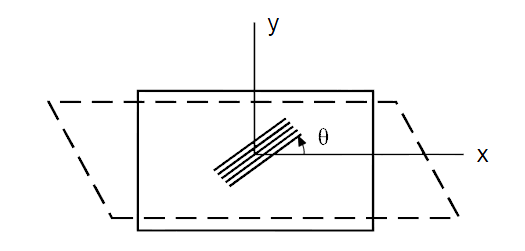
\includegraphics{../images/fiber_shear.PNG}
\caption{image}
\end{figure}

\begin{figure}
\centering
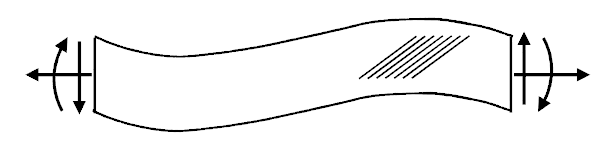
\includegraphics{../images/fiber_warp.PNG}
\caption{image}
\end{figure}
\end{frame}

\begin{frame}{tensile testing}
\protect\hypertarget{tensile-testing-2}{}
\begin{figure}
\centering
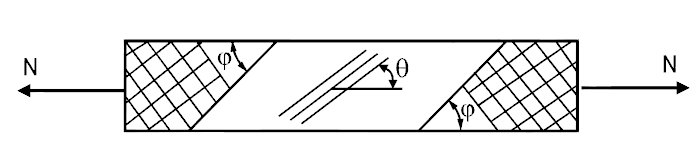
\includegraphics{../images/oblique_tabs.PNG}
\caption{Oblique tabs developed by Sun and Chung in 1993}
\end{figure}
\end{frame}

\begin{frame}{shear testing}
\protect\hypertarget{shear-testing}{}
\begin{itemize}
\tightlist
\item
  Just as grip constraints can make a state of pure tension difficult to
  obtain, it can be difficult to obtain a pure state of shear
\item
  There are many different shear test methods for anisotropic materials,
  most involve specialized grips and specialized specimen geometry
\end{itemize}
\end{frame}

\begin{frame}{iosipescu shear}
\protect\hypertarget{iosipescu-shear}{}
\begin{figure}
\centering
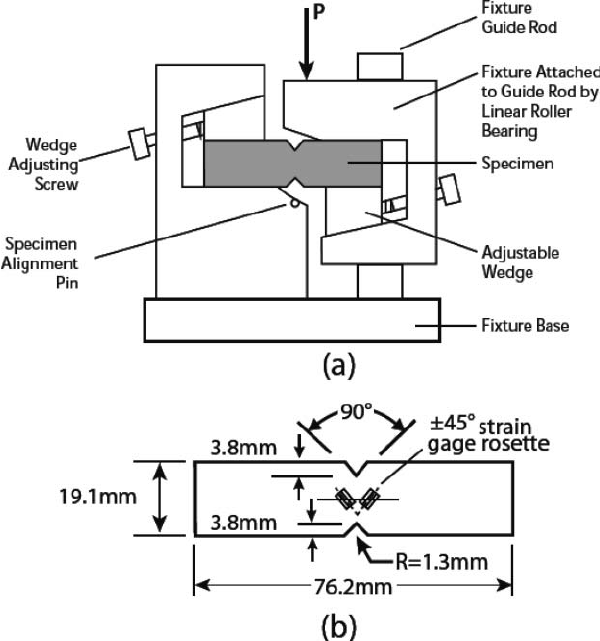
\includegraphics{../images/iosipescu.png}
\caption{image}
\end{figure}
\end{frame}

\begin{frame}{two-rail shear}
\protect\hypertarget{two-rail-shear}{}
\begin{figure}
\centering
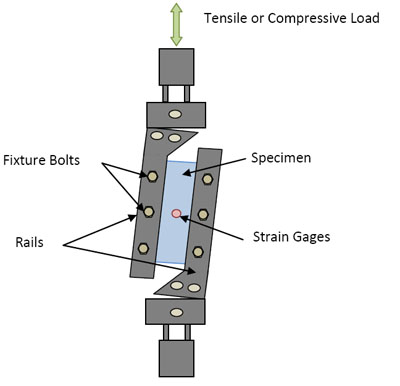
\includegraphics{../images/two-rail.jpg}
\caption{image}
\end{figure}
\end{frame}

\begin{frame}{review}
\protect\hypertarget{review}{}
\begin{itemize}
\tightlist
\item
  Group 1: How many (theoretically) tests required to characterize a
  monoclinic material
\item
  Group 2: How many (theoretically) tests to characterize an orthotropic
  material
\end{itemize}
\end{frame}

\begin{frame}{reading for next class}
\protect\hypertarget{reading-for-next-class}{}
\begin{itemize}
\tightlist
\item
  Analytic techniques for anisotropic elasticity:
  \href{http://solidmechanics.org/text/Chapter5_5/Chapter5_5.htm}{link}
\item
  Large Deformation - pp.~334 - 349
\end{itemize}
\end{frame}

\end{document}
